\section{Exploration of New Algorithms}

To enable the creation of an interactive analysis, 
reasoning, and discovery environment, new methodologies are needed to
detect and effectively presentation the scientifically interesting data
buried in large ALMA data cubes.
The fundamental fact is that most of the pixels in any data cube are noise,
and data cubes with significant signal density (many lines and/or many spatial
features) are difficult to mine for science content. 

Much of the science with large data cubes to date has been accomplished with
simple information compression techniques: moment maps, velocity position
diagram along selected axes, rotation curve fitting, and visual inspection
for eye-catching correlations. Analysis such as principle component 
analysis and other orthogonal component decomposition analysis have been
applied for analyzing structure in complex environments such as molecular
cloud. In general, however, the generally available techniques in standard
radio astronomy data reduction packages have not change in major ways in
over 20 years.

As a part of this study, we have looked at the kinds of new analysis tools
will be of high value to astronomy for: (1) comparing the characteristic
of emission within a given line at different velocities, in  different lines,
for the same line in different sources. The subsections below discuss two
specific examples that we explored at the level of creating prototype tools.

\subsection{Overlap Integral}

The overlap integral provides an overview of the emission properties across
a number of spectral lines; it can also be generalized to apply
to the emission as a function of velocity within a line or across source. 
In the multi-line application,
for each detected line, one assigns a one or zero indicating the presence of emission
at some selected level, and
then logically ORs them across all lines, creating a bit-mask map of the emission
present in each spatial-velocity pixel. One can do this in a moment map, or a cube, to determine in
which spatial or velocity regions certain lines are present or absent in relation to
other lines. 

The final image or cube is a integer map with 0/1 in each bit representing the presence/lack
of emission in one of the lines. This integer is then easily displayed as a color image.
An example using NGC 253 spectral line data from ALMA Cycle 0 is
shown in Figure 9. This technique can also be applied to individual channels of
a single spectral line to examine the velocity pattern of emission, similar to a renzogram.

\begin{figure}[t]
\centering
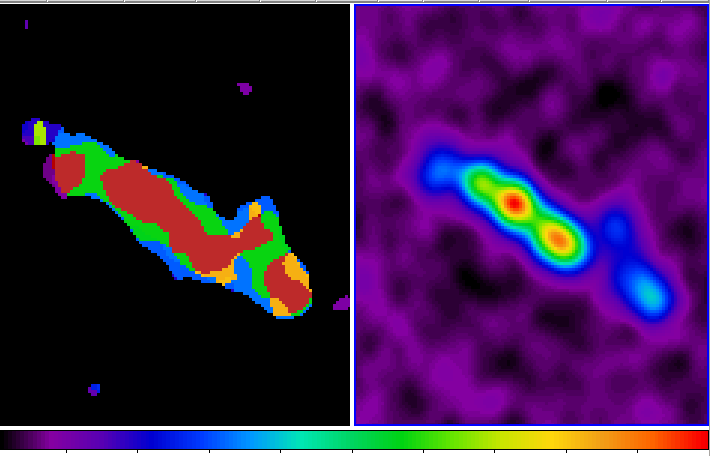
\includegraphics[width=0.75\textwidth]{overlap.png}
\hspace{0.03in}
\caption{\small \setlength{\baselineskip}{0.85\baselineskip}
An example of an overlap integral using ALMA Cycle 0 data of NGC~253. Right: Integrated flux
(moment zero) image of the CO J=1-0 emission. Left: The combined overlap integral -- valued from
0 to 255 -- of 8 spectral lines. Each line is represented by a single bit in an 8-bit
integer which is then translated into a color scale. As can be seen, most of the peaks
have all 8 lines present (red). The spectral lines used to create this overlap integral are
CO, C$^{17}$O J=1-0, CN J=1-0 F=1, CN J=1-0 F=2, HC$_{3}$N, CH$_{3}$OH, H$_2$CS,
and CH$_{3}$C$_{2}$H.
  }
\label{fig:hst}
\end{figure}

\subsection{Descriptor Vectors}

One technique from computer science with significant potential for implementation
in astronomy is "descriptor vectors". The approach is to segment an image or
cube and and calculate an n-dimensional description vector to characterize each
segment. One of the current applications of this technique in visual image analysis
is in automated feature identification. In this application, the image is segmented
into M-regions and each region is characterized by an n-dimensional vector which
might simply the intensity distribution of the pixels within the segment, or the
pixel color distribution, or contrast level; it could be that the segment is characterized
by the spatial shape distribution. Once the vectors are generated, then it is
easy to calculate the "distance" between the various vectors and to identify
which vectors are most like, or unlike, each other. One can identify clusters
of vectors. This gives you an ordered list of locations in the image or cube
that share similar characteristics.

The descriptor vector approach
provides an application-independent, purely mathematical measurement of information 
(M. Chen and H. Janicke. ``An information-theoretic framework for visualization''
IEEE Transactions on Visualization and Computer Graphics, 16(6):1206 –1215, 2010;
H. Janicke and M. Chen. ``A salience-based quality metric for visualization''
Computer Graphics Forum, 29(3):1183–1192, 2010).  
For astronomical images, description vectors can be chosen from any number of 
properties of the emission.  An example in vision research utilizes a color 
histogram, which enables a very fast cataloging of feature types in an image, 
as well as finding the features similar to a selected one, a type of machine learning 
(C. Y. Ip and A. Varshney, ``Saliency-assisted navigation of very large landscape 
images'', IEEE Transactions on Visualization and Computer Graphics, 17(12):1737– 1746, 2011;
C.Y. Ip, Ph.D. Thesis, University of Maryland, 2014).
We have imported several astronomical data cubed into existing descriptor vector
software associated with the work by Mr. Ip (UMD computer science graduate student)
and Professor Amitabh Varshney (UMD Professor in computer science).  One of the
aspects of the descriptor vector method is that you have a set mechanism for
how to proceed but you have wide latitude in how you segment the image and the
mathematical prescription for calculating the n-dimensional vector. This makes
the method very versatile.

It is important to note that
although this may sound similar to Principal Component Analysis, the descriptive 
vectors do not need to be orthogonal or even have the same units. Because of the
versatility and the specific focus possible with tuned vector formulations,
data mining with this technique can be an extremely powerful, allowing a 
fast comparison of features that might be missed otherwise.  

During our study, we evaluated this technique’s 
potential for achieving astronomical science goals.  The key to success is discovering the best 
description vector for the specific science case (M. Chen and H. Janicke. ``An 
information-theoretic framework for visualization'', IEEE Transactions on Visualization 
and Computer Graphics, 16(6):1206 –1215, 2010).   For example, in one case 
the descriptive vector that best describes a specific science goal may be the properties 
of the certain molecular lines and the overlap interval, while another may be the 
location of the molecular peaks with respect to the continuum.  ADMIT can provide the 
infrastructure to write various descriptor vectors, provide some of the vectors 
(based on BDPs) that will most likely to cover standard science goals, and provide a 
task that determines best vector choices based on user inputs.   
We will also document the descriptor formulation procedure so that users have the 
option to build on this approach in the future.   

There are, of course, no significant barriers to generalizing this approach to
comparing multiple lines or multiple sources. For example to be able to ask questions
like: Where in my data cubes to HCN and CO have overlapping emission but there
is no HNC emission? Give me a list of all of the position-position-velocity locations
were SO and SiO emission are coming from the same locations. Or, give me a list
of the places where the CO is falling off rapidly with velocity and there is
SO emission.

\subsection{Learning Algorithms}

In computer science applications, the descriptor vector characterization of an image
can be layered with learning algorithms which can power efficient data mining. The
simplest application is to make a descriptor vector description of an image or
cube then to manual look at the image or cube and identity a region of interest.
The algorithm can then calculate which other segments have similar vectors to your
selected regions, providing an ordered list of the 10 nearest vectors. One can
then view those regions, select which ones are correctly of interest; feed the
new set of regions if interest into the algorithm and get a new ordered list of
most similar vectors/regions. 

This combination of compact description approach and learning-selection is very
well suited for combination with a visualization tool. The algorithms here 
provide a computing layer which provide an order list of interested regions in the
cube for display in the visualization tool. The visualization give the user
rapid feedback to refine the search; the list of preferred regions is feed back
into the algorithm for an increasingly targeted search.
